\chapter{Extracting Load Features}
The math model presented in the Chapter 3 requires as input the power level, the minimum running time and sequence of states for each load. This chapter presents the methodology that was applied for extracting these features in both a supervised setting and an usupervised setting. As a difference, in the supervised setting, these features are extracted from the measurements of each appliance alone. In the unsupervised setting, those features are extracted from snippets from the total power signal. More details are presented in each subsection. 


\section{Supervised Setting}

This section proposes an algorithm to create the load signatures. This algoritm extract the most relevant power states of the load. First let’s start with an example. We begin with the following question: how do we create a mathematical model for the load of the figure 1?

\begin{figure}[tb]
    \centering
    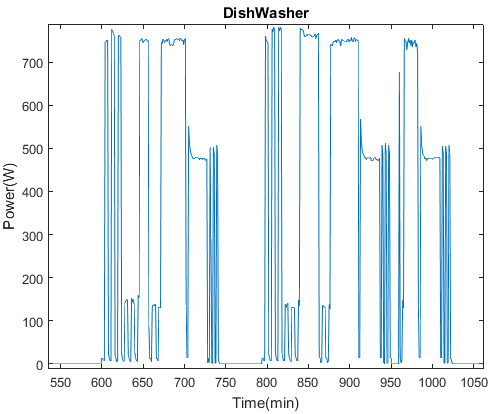
\includegraphics[width=1\columnwidth ]{1.png}
    \caption{Power measurement of DishWasher}
    \label{ch31}
\end{figure}

First, let’s take a look on the histogram:
\begin{figure}[tb]
    \centering
    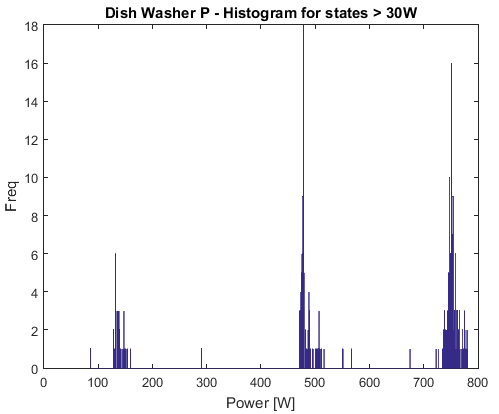
\includegraphics[width=1\columnwidth ]{2.png}
    \caption{Histogram of DishWasher}
    \label{ch32}
\end{figure}


This histogram tells us that there are 3 main power states when the DishWasher is on. Hence, we can build a model for this load by using a clustering algorithm. 

\begin{figure}[tb]
    \centering
    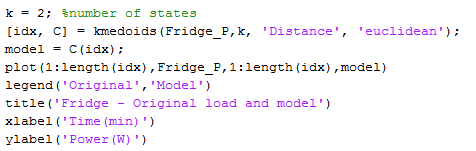
\includegraphics[width=1\columnwidth ]{3.png}
    \caption{Cluster algorithm}
    \label{ch33}
\end{figure}

The next figure shows the model created by using a median clustering algorithm:

\begin{figure}[tb]
    \centering
    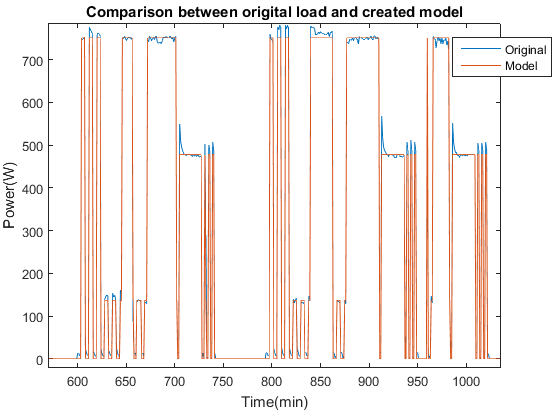
\includegraphics[width=1\columnwidth ]{4.png}
    \caption{Model based on clusters from the histogram}
    \label{ch34}
\end{figure}

Then, the atributes state, mindisc and ant are loaded to the model. The next figures present the other models that are considered for the system 2. 
\begin{figure}[tb]
    \centering
    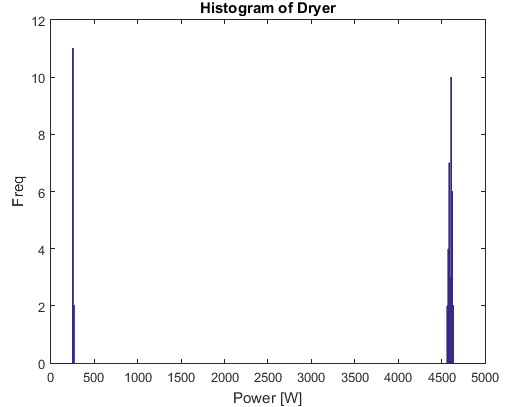
\includegraphics[width=1\columnwidth ]{5.png}
    \caption{Model based on clusters from the histogram}
    \label{ch35}
\end{figure}


\begin{figure}[tb]
    \centering
    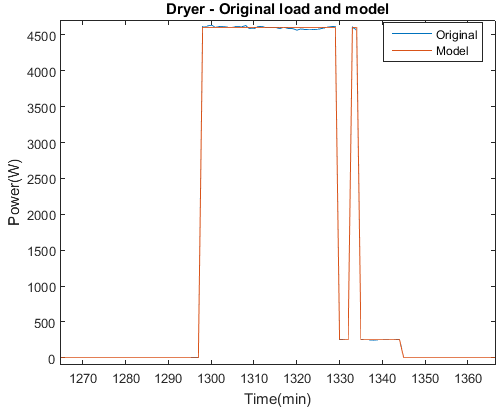
\includegraphics[width=1\columnwidth ]{6.png}
    \caption{Model based on clusters from the histogram}
    \label{ch36}
\end{figure}


\begin{figure}[tb]
    \centering
    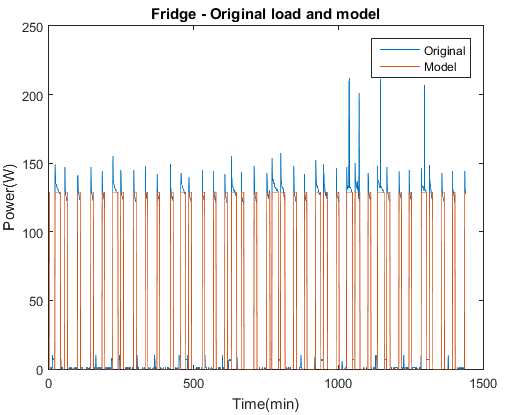
\includegraphics[width=1\columnwidth ]{7.png}
    \caption{Model based on clusters from the histogram}
    \label{ch37}
\end{figure}

the following figure shows the model of the fridge with 4 states

\begin{figure}[tb]
    \centering
    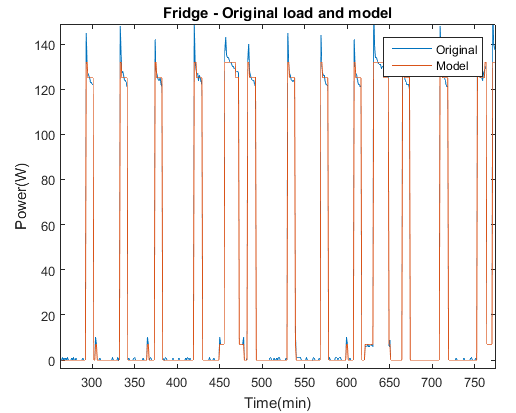
\includegraphics[width=1\columnwidth ]{8.png}
    \caption{Model based on clusters from the histogram}
    \label{ch37}
\end{figure}

\section{Unsupervised Setting}


\section{Summary}

Ideas:
- "Using the total power signal, we extract all snippets of data where consumption increase over some th then eventually returns to its original level; some of these are indecpherable due to the aggregation, but especially for short device durations there are occasional snipptes of individual devices. We model all these snippets as empirical HMM (means equal to the observed output and transition probabilities set based upon the amount of time spent at each power level) and looked at all pairwise probabilities between them (the probability of one snippet generating another); using the k-nearest-neighbor graph induced by these probabilities, we ran spectral clustering to group devices together. This resulted into nine prototypical motifs, " - Kolter